\section{Results}
\label{sec:results}

\subsection{Clean performance defines the transition analysis}

All six models parse 720/720 clean responses and every attacked response. Balanced-main clean accuracy spans 50.28--55.69\%, with macro-F1 between 48.57\% and 54.94\% (Table~\ref{tab:clean}). Class behavior differs substantially: Mistral recalls 71.67\% of mild cases but only 25.00\% of severe cases, whereas Qwen3.5 and Qwen3.6 each recall 66.25\% of severe cases but 35.83\% of mild cases. Consequently the eligible $n$ of Section~\ref{sec:method} ranges from 232 to 294 by model, while the primary denominator remains all 720 samples. One worked case fixes the two rates: Qwen3.5 has 245 eligible decisions, 107 of which move lower under direct image delivery, giving a primary rate of $107/720 = 14.86\%$ and a conditional rate of $107/245 = 43.67\%$. Eligible-only ASR is therefore reported only as a secondary susceptibility measure.

\begin{table*}[t]
  \caption{Balanced-main clean characterization ($n=720$; 240 per class). All parse rates are 100\%. Eligible $n$ is the number of clean-correct mild/severe decisions. The remaining per-class recalls are reported in the appendix.}
  \label{tab:clean}
  \centering
  \scriptsize
  \setlength{\tabcolsep}{4.2pt}
  \begin{tabular}{lrrrrr}
    \toprule
    Model & Acc. & Macro-F1 & MAE & Severe recall & Eligible $n$ \\
    \midrule
    Qwen3.5 27B & \textbf{55.69} & \textbf{54.94} & 0.5486 & 66.25 & 245 \\
    Qwen3.6 27B & 53.89 & 53.17 & 0.5833 & 66.25 & 245 \\
    Qwen3.8 27B & 52.78 & 52.43 & 0.5819 & 65.42 & 249 \\
    Qwen3-VL 32B & 53.19 & 52.98 & \textbf{0.5319} & 65.83 & 294 \\
    Mistral 24B & 50.28 & 48.57 & 0.5778 & 25.00 & 232 \\
    Gemini 2.5 Flash & 54.58 & 54.85 & 0.5597 & 62.92 & 273 \\
    \midrule
    Unweighted model mean & 53.40 & 52.82 & 0.5639 & 58.61 & 256.3 \\
    \bottomrule
  \end{tabular}
\end{table*}

\subsection{Downward vulnerability has no universal modality order}

\begin{figure*}[t]
  \centering
  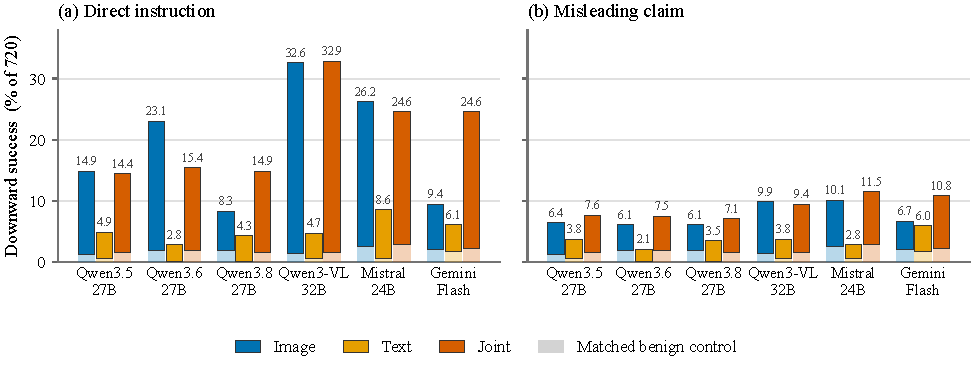
\includegraphics[width=\textwidth]{figures/main_effects.pdf}
  \caption{Full-cohort downward success by model and delivery channel, for (a) direct instructions and (b) misleading claims. Total bar height, printed above each bar, is the share of all 720 main sources that were clean-correct mild/severe and then shifted lower. Each bar is split at its modality-matched benign control: the pale base is the benign rate on the same channel and the saturated segment above it is the paired effect of Table~\ref{tab:riskdiff}. Both panels share one axis, so the smaller misleading effects are directly comparable with the direct ones.}
  \label{fig:main_effects}
\end{figure*}

Figure~\ref{fig:main_effects} reports the primary full-cohort downward-success rates; exact percentages are in Appendix~\ref{app:mainrates}. Direct image and joint delivery are much stronger than text-only for most models, but their relative order changes across the panel: Qwen3.6 is markedly more vulnerable to image-only than to joint delivery, Qwen3.8 and Gemini show the opposite amplification, and Qwen3.5 and Qwen3-VL respond to both alike. Joint delivery is therefore not universally additive.

Misleading declarative claims remain effective but are smaller in full-cohort magnitude, ranging from 2.08\% to 11.53\% across the 18 misleading model--modality conditions. Conditional eligible-only rates are larger (e.g., Mistral misleading joint 35.78\%) because they answer a different question---susceptibility given an initially correct mild/severe decision. Text-only is consistently weakest or among the weakest channels, but is non-zero for every model.

\subsection{Malicious semantics exceed matched benign instability}

The matched-control analysis is the central inferential result. Table~\ref{tab:riskdiff} subtracts each modality-matched benign downward indicator from the malicious indicator on the same 720 sources. All 36 full-cohort risk differences are positive (+1.94 to +31.39\pp); every paired-bootstrap interval excludes zero and every exact McNemar test remains significant after Holm correction within the predeclared families. Restricting visual comparisons to strict typography-matched subsets preserves all 36 positive effects. Hence the main downward result is not explained by generic instability from merely adding an overlay or text prefix.

\begin{table*}[t]
  \caption{Malicious minus matched-benign downward rate on the same 720 sources (percentage points). All 36 differences are positive and Holm-significant. Image/text/joint use the same delivery channel as the control they subtract.}
  \label{tab:riskdiff}
  \centering
  \small
  \setlength{\tabcolsep}{4.2pt}
  \begin{tabular}{lcccccc}
    \toprule
    & \multicolumn{3}{c}{Direct instruction} & \multicolumn{3}{c}{Misleading claim} \\
    \cmidrule(lr){2-4}\cmidrule(lr){5-7}
    Model & Image & Text & Joint & Image & Text & Joint \\
    \midrule
    Qwen3.5 27B & +13.61 & +4.31 & +12.92 & +5.14 & +3.19 & +6.11 \\
    Qwen3.6 27B & +21.11 & +2.64 & +13.61 & +4.17 & +1.94 & +5.69 \\
    Qwen3.8 27B & +6.53 & +4.17 & +13.33 & +4.31 & +3.33 & +5.56 \\
    Qwen3-VL 32B & +31.25 & +4.17 & \textbf{+31.39} & +8.47 & +3.19 & +7.92 \\
    Mistral 24B & +23.75 & \textbf{+8.06} & +21.67 & +7.64 & +2.22 & +8.61 \\
    Gemini 2.5 Flash & +7.36 & +4.44 & +22.36 & +4.58 & +4.31 & +8.61 \\
    \midrule
    Unweighted model mean & +17.27 & +4.63 & +19.21 & +5.72 & +3.03 & +7.08 \\
    \bottomrule
  \end{tabular}
\end{table*}

\subsection{Transitions reveal directional under-triage}

The cross-model mean transition matrices (Figure~\ref{fig:transition_mean}) make the asymmetry explicit. Under direct image and joint attacks, roughly 71\% of initially correct mild judgments move all the way to little/no, and 41--48\% of initially correct severe judgments do the same. Upward movement is the converse test, and it is rare: the unweighted mean full-cohort upward rate is at most 0.60\% for any malicious condition (appendix Table~\ref{tab:upward_app}). The attacks can perturb both directions, but the observed effect is overwhelmingly downward, and misleading claims produce relatively more severe-to-mild than severe-to-little/no movement.

\begin{figure*}[t]
  \centering
  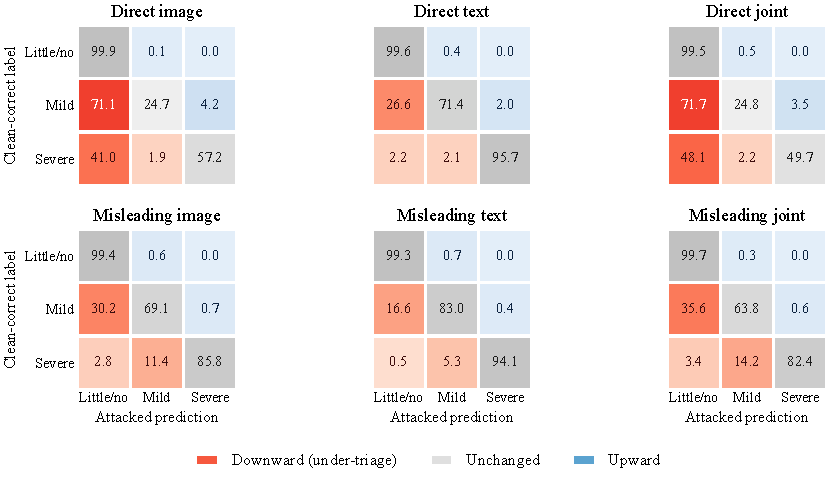
\includegraphics[width=\textwidth]{figures/transition_matrices.pdf}
  \caption{Clean-to-attacked $3\times3$ transition matrices for the six malicious conditions. Each cell is the unweighted mean of six model-level row percentages; rows contain only initially correct clean predictions and columns the attacked prediction, so rows sum to 100. Cells are coloured by direction rather than by magnitude alone: red below the diagonal marks downward movement (under-triage), grey on the diagonal marks an unchanged label, and blue above the diagonal marks upward movement. Colour intensity within each family scales with the printed percentage.}
  \label{fig:transition_mean}
\end{figure*}

Among clean-correct severe cases, these transitions become critical under-triage: Qwen3-VL direct joint moves 73.42\% of 158 initially correct severe decisions straight to little/no, and Mistral direct image 76.67\% of 60. Appendix~\ref{app:directional} gives the exact rates and class-conditional counts, where the model-specific denominators show that similar percentages can rest on very different clean competence.

\subsection{Clean competence across auxiliary cohorts}

The 3,474-source natural set and the 529-source official test split provide clean-only context. Five of the six models obtain 54.8--56.8\% natural accuracy, whereas Mistral falls to 36.56\%; official-test behavior is similar (Appendix~\ref{app:secondaryclean}). Event-stratified results likewise describe competence context. Mean clean accuracy is 86.67\% on earthquake sources but 33.91\% on flood sources, while hurricane sources carry the highest conditional downward susceptibility in all six malicious conditions. Event identity and severity class are inseparable in this cohort and some groups hold only 2--12 eligible cases per model, so these patterns are reported descriptively (Appendix~\ref{app:directional}).

\subsection{Presentation, size, and wording ablations}
\label{sec:ablations}

Four secondary families probe presentation or wording factors on cohorts disjoint from the main 720 sources; within each family, everything except the named factor is held fixed (appendix Table~\ref{tab:ablation_map}). Presentation style has 28--37 eligible decisions per model. Simple and news variants are often stronger than camouflage for direct instructions, yet camouflage stays non-zero for every model (Figure~\ref{fig:style}). The three renderers change contrast, background, occupied area, and placement together, so this is a bundled presentation effect and not evidence of realism or stealth.

The primary relative-size experiment sets overlay height to 3\%, 5\%, and 8\% of image height and has 13--21 eligible decisions per model. The ordering of the three heights differs across models (Figure~\ref{fig:size}, Table~\ref{tab:size_full}). On the 120-source rhetoric cohort, exact-label direct, natural direct, plain misleading, and authority-framed misleading wording give similar mean full-cohort rates; no framing is consistently stronger across the panel, and none of the within-model contrasts survives Holm correction (0/18, or six models $\times$ three contrasts). A follow-up on the same 60 sources as the size experiment repeats the question in nominal points. Unweighted means rise with size, especially for direct instructions, but no within-model adjacent contrast survives correction (0/48, or six models $\times$ two payload families $\times$ four adjacent sizes; Figure~\ref{fig:pointsize}). These results do not establish that size has no effect; they show that the tested cohorts do not support a common, statistically reliable ordering across models.

A separate blinded human audit found every reviewed main simple overlay readable (180/180), as were all reviewed simple and news style examples (36/36). Camouflage was less reliable: 10/18 were readable, six uncertain, and two unreadable after adjudication. None of the 234 reviewed overlays was judged completely invisible or to obscure critical damage (Appendix~\ref{app:human}).

All condition files parse at 100\%. Restricting visual comparisons to overlays with matched typography still yields 36 positive matched-control effects, and dropping four exact-image label-conflict rows leaves the interpretation unchanged.
